\documentclass[runningheads]{llncs}
\usepackage[T1]{fontenc}
\usepackage{graphicx}
\usepackage{booktabs}
\usepackage{amsmath,amssymb}
\usepackage{microtype}
\usepackage{url}
\usepackage{xurl}
\usepackage{cite}
\usepackage{xcolor}

\InputIfFileExists{generated/macros.tex}{}{}
\providecommand{\PlattAlpha}{1.40}
\providecommand{\PlattBeta}{-0.68}

\newcommand{\logit}{\operatorname{logit}}
\newcommand{\clip}{\operatorname{clip}}

\pdfinfoomitdate=1
\pdftrailerid{}
\pdfsuppressptexinfo=-1
\begin{document}
\title{CARF: Bounded Anchored Fusion for Multimodal Prediction with Unreliable Modalities}
\titlerunning{CARF: Bounded Anchored Fusion}
\author{Anonymous Authors}
\authorrunning{Anonymous Authors}
\institute{Anonymous Institution}
\maketitle

\begin{abstract}
Multimodal predictors are often deployed where some inputs are always collected while others are optional or fragile. For instance, in breast cancer treatment planning, clinical variables are recorded for every patient, whereas gene expression and imaging may be missing, acquired on a different platform, or corrupted. We propose a method called Clinical-Anchored Residual Fusion (CARF) that keeps the clinical model's logit as a fixed anchor and lets optional experts shift it only within a fixed log-odds budget. CARF returns the clinical prediction exactly when optional inputs are absent and bounds the effect of each modality on the output; its six nonnegative gate coefficients are fitted with a convex objective over all missingness patterns and a smoothed worst case over expert corruptions. We evaluate CARF on 976 I-SPY2 and 112 I-SPY1 patients against stacking, offset logistic regression, and neural fusion baselines. At comparable external discrimination (AUROC \ExtCarf{} versus \ExtStack{} for stacking), CARF loses the least AUROC relative to the clinical model among the fusion baselines when the transcriptomic expert becomes uninformative (\RnaPermCarf{} versus \RnaPermStack{} for stacking and \RnaPermOffset{} for offset logistic regression, with paired bootstrap intervals against stacking, mask-stacking, and a ModDrop network that exclude zero), and its prediction never moves by more than \MaxDispCarfAll{} logits from the clinical one. The robust objective also transfers to offset logistic regression, whereas only the bounded rule gives a per-patient guarantee. On a further independent breast cancer cohort, CARF matches the clinical model when the transcriptomic input is corrupted.
\keywords{Multimodal learning \and Missing modalities \and Robust fusion \and Convex optimization \and Bounded influence}
\end{abstract}

%======================================================================
\section{Introduction}

Multimodal learning combines heterogeneous sources of information about the same individual \cite{baltrusaitis2019}. In many applications, the modalities do not play symmetric roles: some inputs are cheap and always recorded, while others are optional, acquired with different protocols at different sites, and can be missing or of poor quality. A fusion model trained on complete data may, however, depend on an optional modality to a degree that is not safe once that modality is absent or corrupted. Stacking \cite{wolpert1992} and learned gates can assign an arbitrarily large weight to an expert which is accurate on the training cohort, and quality scores do not remove this risk, as an incorrect expert can be highly confident.

We study this problem in the prediction of pathological complete response (pCR), i.e., no invasive cancer at surgery after neoadjuvant chemotherapy. I-SPY1 \cite{esserman2012} and I-SPY2 \cite{wolf2022ispy} are public breast cancer trial cohorts in which each patient has clinical variables, pretreatment gene expression, and contrast-enhanced MRI. Clinical variables such as hormone-receptor and HER2 status are available for every patient, while expression and imaging are optional.

To address this problem, we propose Clinical-Anchored Residual Fusion (CARF), a late-fusion rule that treats the always-available modality as an anchor and restricts how far the optional modalities can move the prediction away from it. In particular: (i) we introduce a fusion rule with an explicit log-odds budget that falls back exactly to the anchor when optional inputs are absent and bounds the effect of each optional modality on the output; (ii) we fit the rule with a convex objective over all missingness patterns and a family of expert corruptions, which applies to any late-fusion rule; and (iii) we compare CARF with stacking, offset logistic regression, and neural fusion baselines on an external cohort, under simulated failures at the expert-output and raw-input level, and on patients with naturally missing modalities.

%======================================================================
\section{Related Work}

ModDrop \cite{neverova2015} trains fusion models to tolerate absent modalities by dropping them during training, but does not limit how much a present but corrupted modality can change a prediction. A recent line of work weights experts by estimated quality: QA-MoE \cite{sun2026} separates quality estimation from expert routing in clinical prediction with noisy and missing modalities, and Moon et al.~\cite{moon2026} question whether such reliability scores actually change downstream decisions. QMF \cite{zhang2023qmf} derives generalization guarantees for uncertainty-weighted late fusion, and offset logistic regression is a standard tool to update clinical prediction models with new predictors \cite{janssen2008}. UCMR-Net \cite{tang2026} is, to the best of our knowledge, the closest existing approach: it adds adaptive nonverbal residuals to a text anchor for sentiment prediction. This approach does not, however, bound the total correction applied to the anchor, and its residual weights are produced by a trained network. In comparison, CARF bounds the total logit correction by construction and fits its gate with a convex cross-fitted objective related to distributionally robust optimization \cite{sagawa2020}, in which the environments are perturbations of the optional experts.

%======================================================================
\section{Approach}

Consider a binary outcome $y$ and experts each trained on one modality. The anchor expert outputs a probability $p_C$ for every patient; in our setting it is the clinical model. The optional experts $j\in\{R,M\}$ (transcriptomic, i.e., RNA, and MRI) output probabilities $p_j$ with an availability indicator $m_j\in\{0,1\}$. Let $a=\logit(p_C)$ be the anchor logit and $d_j=\logit(p_j)-a$. We seek a fusion rule that (i) returns $a$ exactly when every optional input is absent, (ii) keeps the fused logit within a known distance of $a$ and bounds the effect of each modality, and (iii) is fitted with a procedure that accounts for missing and corrupted optional inputs.

\subsection{Anchored residual fusion}

For each optional expert, CARF clips the logit difference to a fixed range $[-B,B]$, i.e., $r_j=\clip(d_j,-B,B)$, and scales it by three context functions with values in $[0,1]$:
\begin{equation}
 h_{j0}=1,\qquad h_{j1}=e^{-|d_j|},\qquad h_{j2}=1-H(p_j)/\log 2,
\end{equation}
where $H(p)=-p\log p-(1-p)\log(1-p)$ is the binary entropy. The term $h_{j1}$ reduces the correction when an expert strongly disagrees with the anchor, while $h_{j2}$ allows a different correction for confident experts. The fused logit is
\begin{equation}
 z_\theta = a + \sum_{j\in\{R,M\}}\sum_{k=0}^{2}\theta_{jk}\, m_j\, h_{jk}\, r_j,
 \qquad \theta_{jk}\ge 0,\qquad \sum_{j,k}\theta_{jk}\le 1 .
 \label{eq:carf}
\end{equation}
A missing modality contributes zero, so that absence is represented by the mask and not by a neutral probability; as the six coefficients are nonnegative, CARF can reduce the influence of an optional expert but cannot reverse its direction (Fig.~\ref{fig:architecture}).

\begin{figure}[t]
\centering
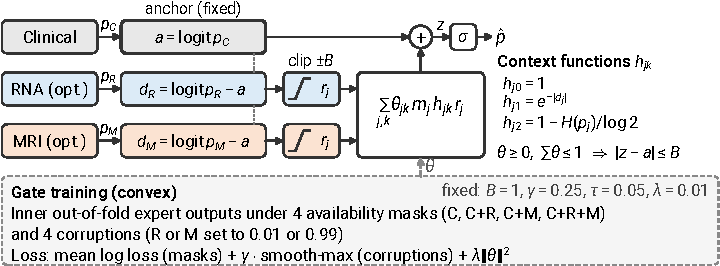
\includegraphics[width=0.86\linewidth]{figures/fig_architecture.pdf}
\caption{CARF with clinical (C), transcriptomic (R), and MRI (M) experts. Optional experts contribute clipped residuals relative to the anchor logit $a$, scaled by context functions $h_{jk}$ and masks $m_j$ and weighted by $\theta\ge0$, $\sum\theta\le1$.}
\label{fig:architecture}
\end{figure}

\subsection{Properties}

Let $b_j=B\sum_k\theta_{jk}$ be the budget of modality $j$ and $b=b_R+b_M\le B$ the total budget. Three properties follow directly from Eq.~\eqref{eq:carf}, since every summand satisfies $|m_jh_{jk}r_j|\le B$ and depends only on expert $j$ and the anchor. \emph{Fallback:} if $m_R=m_M=0$, then $z_\theta=a$. \emph{Bounded displacement:} for any optional inputs, $|z_\theta-a|\le b$, and hence $|\hat p-p_C|\le b/4$, as the slope of the sigmoid is at most $1/4$. Replacing or removing modality $j$ alone, while holding the other inputs fixed, changes $z_\theta$ by at most $2b_j$. \emph{Ranking certificate:} two patients whose anchor logits differ by more than $2b$ keep their anchor ordering for any values of the optional inputs. All three statements also hold with the sharper budget $b^*_j=B\theta_{j0}+\kappa\theta_{j1}+B\theta_{j2}$, since $|e^{-|d|}\clip(d,-B,B)|\le\kappa=\max_{t\le B}te^{-t}$, which equals $e^{-1}$ for $B\ge1$.

\subsection{Convex robust gate fitting}

The gate is fitted on out-of-fold expert predictions obtained by five-fold cross-fitting within the training set. Let $L_e(\theta)$ be the mean logistic loss of $z_\theta$ in environment $e$. The set $\mathcal M$ contains the four combinations of optional availability, and the set $\mathcal C$ contains four corruption environments in which one optional expert is replaced by $0.01$ or $0.99$. We minimize
\begin{equation}
 \min_{\theta\ge0,\ \mathbf 1^\top\theta\le1}\;
 \frac14\sum_{e\in\mathcal M}L_e(\theta)
 +\gamma\,\tau\log\Big(\frac14\sum_{e\in\mathcal C}e^{L_e(\theta)/\tau}\Big)
 +\frac\lambda2\|\theta\|_2^2 .
 \label{eq:objective}
\end{equation}
The second term is a smoothed maximum over corruption environments with temperature $\tau$. Since $z_\theta$ is linear in $\theta$ for fixed expert outputs, each $L_e$ is convex, and so are the log-sum-exp term and the penalty: the problem is convex over a polytope, strictly convex for $\lambda>0$, and we solve it with sequential least-squares programming. We fix $B=1$, $\gamma=0.25$, $\tau=0.05$, and $\lambda=0.01$ and do not tune them on either cohort.

\paragraph{Post-hoc calibration.} As the experts use class-balanced weights, we optionally apply Platt scaling \cite{platt1999}, $\hat p=\sigma(\alpha z_\theta+\beta)$, fitted on inner out-of-fold CARF logits. As the fitted slope is positive, the map is monotone: rankings and the ranking certificate are unchanged, and the other properties hold with respect to the recalibrated anchor $\alpha a+\beta$ with the bound scaled by $\alpha$ (here $\alpha=\PlattAlpha$).

%======================================================================
\section{Experiments}

\subsection{Experimental setup}

\paragraph{Data.} We use \NDev{} I-SPY2 patients (\NDevPos{} with pCR) for development and \NExt{} I-SPY1 patients (\NExtPos{} with pCR) as an external cohort. Each patient has clinical variables (age, hormone-receptor and HER2 status), pretreatment microarray expression (Gene Expression Omnibus GSE194040 for I-SPY2 \cite{wolf2022ispy} and GSE22226 for I-SPY1), and pretreatment contrast-enhanced MRI with tumor masks from the BreastDCEDL release \cite{fridman2026} of the TCIA collections \cite{tciaispy1,tciaispy2}. Expression is restricted to the \NGenes{} genes shared by both platforms and rank-normalized within each patient.

\paragraph{Experts.} Each expert is a class-balanced logistic regression with fixed hyperparameters: on the three clinical variables, on 250 genes selected within each training set by variance and an ANOVA test, and on \NMriFeat{} fixed intensity, shape, kinetic, and texture features computed inside the tumor mask (details in the supplementary material). All preprocessing is fitted within each training partition.

\paragraph{Protocol.} Internal evaluation uses five repeats of stratified five-fold cross-validation on I-SPY2; in each outer training set, inner cross-fitting produces the expert predictions used to fit every fusion model, and the external models are fitted in the same way on all of I-SPY2. I-SPY1 labels are used for neither fitting nor hyperparameter choice.

\paragraph{Baselines.} All fusion models receive the same expert probabilities. We compare with the individual experts; the mean of available probabilities; stacking \cite{wolpert1992}, i.e., logistic regression on the three probabilities; mask-stacking, i.e., stacking trained on all four availability masks with explicit indicators; offset logistic regression, which fits the RNA and MRI logits and a free intercept with the clinical logit as a fixed offset, without class weights, and an $\ell_2$ penalty; and a ModDrop-style MLP \cite{neverova2015} trained on all four masks, with architecture chosen by inner cross-validation. CARF ablations remove the robust term ($\gamma=0$), keep only the constant context function (constant basis), or remove both clipping and the budget constraint (unbounded), and we also train offset logistic regression with the robust objective of CARF (robust offset LR).

\paragraph{Metrics and stress tests.} We report AUROC, Brier score, expected calibration error (ECE, in the supplementary material) \cite{guo2017}, and paired bootstrap intervals (2{,}000 resamples) for external AUROC differences. Stress tests freeze all models and alter one optional modality of the external patients, with 30 seeds each. At the output level, we permute the expert probability across patients, a corruption not used in training (the training corruptions and Gaussian noise are reported in the supplementary material). At the input level, we remove 50\% of the genes of each patient, shift 25\% of the genes by two log-ratio units, add noise of one training SD to the MRI features, or remove 60\% of them. Stress intervals resample patients with the 30 realizations held fixed. Refitting the whole pipeline on permuted I-SPY2 labels yields $p=\PermPCarf$ for the external AUROC of CARF, the smallest value attainable with \NPerm{} permutations.

\subsection{Discrimination and calibration}

\begin{table}[t]
\centering
\caption{Discrimination, robustness, and displacement. Internal AUROC: mean $\pm$ SD over the 25 outer folds on I-SPY2. External metrics on the \NExt{} I-SPY1 patients (higher AUROC is better). $\Delta$AUROC: CARF minus the model, 95\% paired bootstrap interval (negative values favor the model). RNA perm.: AUROC with the transcriptomic output permuted (mean of 30 realizations). $\max|z-a|$: largest change of the logit from the clinical anchor over all stress scenarios (lower is better). Bold: best among the fusion baselines and CARF; single experts and ablations are shown for reference.}
\label{tab:main}
\InputIfFileExists{generated/tab_main.tex}{}{\textit{[table pending]}}
\end{table}

On the external cohort (Table~\ref{tab:main}), CARF reaches an AUROC of \ExtCarf{}, compared with \ExtClin{} for the clinical expert, \ExtStack{} for stacking, \ExtMaskStack{} for mask-stacking, and \ExtOffset{} for offset logistic regression; the paired intervals against all fusion comparators include zero, i.e., on 112 patients, the external AUROC of CARF cannot be distinguished from that of the unconstrained fusion rules. Internally, CARF reaches \IntCarf{} and stacking \IntStack{}. The clinical expert is stronger externally than internally, likely because of the unmodeled I-SPY2 treatment arms. The constant-basis (\ExtNoContext{}) and unbounded (\ExtUnbounded{}) ablations match full CARF, and removing the robust term raises the external AUROC to \ExtNoRobust{}, a gain which is lost under transcriptomic failure (Section~\ref{sec:stress}). With regard to calibration, all class-balanced models overestimate the prevalence; when every model is Platt-scaled on its own inner out-of-fold predictions, CARF reaches a Brier score of \PlattBrierCarf{}, comparable to stacking (\PlattBrierStack{}) and mask-stacking (\PlattBrierMaskStack{}).

\subsection{Modality failure}
\label{sec:stress}

\begin{table}[t]
\centering
\caption{External AUROC under failure of one optional modality (mean of 30 realizations). Output-level corruptions permute the expert probability across patients; input-level corruptions alter the expert's inputs. The clinical expert alone reaches \ExtClin{}. $\Delta$ perm.: CARF minus model under RNA permutation, 95\% paired bootstrap interval (all scenarios in the supplement). Bold: best among the fusion baselines and CARF.}
\label{tab:stress}
\small
\InputIfFileExists{generated/tab_stress.tex}{}{\textit{[table pending]}}
\end{table}

When the transcriptomic output is permuted across patients (Table~\ref{tab:stress}), the modality carries no information, and an ideal fusion rule would match the clinical expert (\ExtClin{}). CARF reaches \RnaPermCarf{}, whereas stacking drops to \RnaPermStack{}, mask-stacking to \RnaPermMaskStack{}, and the ModDrop MLP to \RnaPermModDrop{}. Unlike on intact data, these differences exceed the sampling uncertainty: all paired intervals in Table~\ref{tab:stress} exclude zero, except that against the robust offset model. Offset logistic regression, which uses the clinical logit as an offset but has no clipping, budget, or robust term, matches CARF on intact data but drops to \RnaPermOffset{}. Within CARF, the robust term is responsible for this behavior (\RnaPermNoRobust{} without it), as it moves the transcriptomic weight onto $h_{R1}$ and lowers the effective budget $b^*_R$ from \SharpBudgetRnaNoRobust{} to \SharpBudgetRna{}. The robust objective, rather than the bounded rule, thus accounts for most of the empirical robustness: offset logistic regression trained with it reaches \RnaPermRobOffset{} under RNA permutation (\RnaPermRobOffsetGOne{} with $\gamma=1$) and 0.702 on the independent cohort of Section~\ref{sec:natural}. What the objective cannot provide is a guarantee for failures outside its training family: the robust offset model still moves individual predictions by up to \MaxDispRobOffsetAll{} logits and shifts predictions without optional inputs by its intercept, whereas CARF returns the clinical prediction exactly and moves any patient by at most \MaxDispCarfAll{} logits, i.e., by at most $b/4\approx0.19$ in probability. We therefore regard the objective as portable, and the bounded rule as the component that turns average robustness into a per-patient certificate.

At the input level, further from the training environments, CARF reaches \GeneDropFiftyCarf{} with half of the genes missing, compared with \GeneDropFiftyStack{} for stacking and \GeneDropFiftyOffset{} for offset logistic regression, and it also stays above stacking and offset logistic regression when MRI features are perturbed (\MriInNoiseCarf{} versus \MriInNoiseStack{} and \MriInNoiseOffset{} with noise). On I-SPY1, CARF remains above the clinical expert in all input-level scenarios. Finally, the largest observed change of the CARF logit from the anchor over all scenarios is \MaxDispCarfAll{}, which equals the sharp budget $b^*=\SharpBudget{}$ (\SharpBudgetRna{} for RNA and \SharpBudgetMri{} for MRI): the displacement bound is attained. For \CertifiedPairsSharp\% of the external patient pairs, the anchor logits differ by more than $2b^*$, so that their ordering cannot be changed by any optional input.

\subsection{Naturally missing modalities}
\label{sec:natural}

In I-SPY1, \NatRnaOnlyN{} further patients have no usable MRI and \NatMriOnlyN{} no expression; we apply the frozen models to them with their true masks. Over all \NatAllN{} patients with at least one optional modality, CARF reaches \NatAllCarf{}, compared with \NatAllClin{} for the clinical expert, \NatAllStack{} for stacking, and \NatAllMaskStack{} for mask-stacking, with paired intervals that include zero (subgroup results in the supplementary material).

\emph{Independent cohort.} We evaluate the frozen models once on GSE25066, a cohort measured on another platform, without its I-SPY1 patients (409 patients, 85 with pCR, no MRI). With a permuted RNA output or half of the genes missing, CARF stays at the level of the clinical expert (0.662 in both cases), whereas offset logistic regression drops to 0.602 under permutation, and the logit of CARF moves by at most 0.48 from the anchor, as opposed to 1.5--6.0 for the other fusion models (supplementary material).

\subsection{Budget and robustness trade-off}

\begin{figure}[t]
\centering
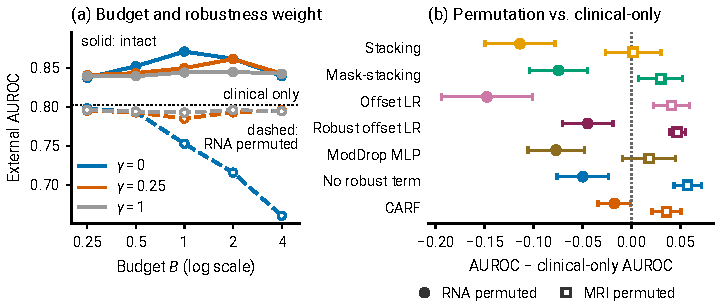
\includegraphics[width=0.84\linewidth]{figures/fig_tradeoff.pdf}
\caption{(a) External AUROC as a function of the budget $B$ for three values of the robust weight $\gamma$, on intact inputs (solid) and with permuted transcriptomic output (dashed). The dotted line is the clinical expert alone. (b) AUROC change relative to the clinical expert when the transcriptomic or MRI output is permuted; error bars show the standard deviation over 30 realizations.}
\label{fig:tradeoff}
\end{figure}

We refit CARF on a grid $B\in\{0.25,0.5,1,2,4\}$ and $\gamma\in\{0,0.1,0.25,0.5,1\}$ (Fig.~\ref{fig:tradeoff}a; supplementary material). For the full model, the coefficients sum to at least 0.99 in every configuration, so that the total budget equals $B$ and is set by the user. Without the robust term, a larger budget increases the damage of a failing modality (at $B=4$, \SweepFourZeroRna{} under RNA permutation, versus \SweepFourQuarterRna{} with $\gamma=0.25$), and a smaller budget without the robust term behaves like our default ($B=0.5$, $\gamma=0$: \SweepHalfZeroClean{} intact, \SweepHalfZeroRna{} permuted): the robust term mainly makes the behavior insensitive to $B$. Selecting $B$ by inner cross-validation picks $B=\CvBMode$ in \CvBCount{} of \CvBFolds{} folds, and the resulting model (\CvExt{} intact, \CvRnaPerm{} RNA-permuted) improves upon the prespecified $B=1$. A synthetic study confirms this (supplementary material).

With the constant context function and no clipping, Eq.~\eqref{eq:carf} reduces to $z=(1-\theta_R-\theta_M)\,a+\theta_R\logit p_R+\theta_M\logit p_M$, a convex combination of logits, so that a large total weight is only useful when the optional experts are stronger than the anchor. On I-SPY2, where the transcriptomic expert is stronger (internal AUROC \IntRna{} versus \IntClin{}), the full gate saturates the constraint, although the constant-basis gate does not (sum \NoContextCoefSum{}); when the anchor dominates, the gate is zero.

\emph{Second domain.} On binary sentiment prediction on CMU-MOSI \cite{zadeh2016mosi} (and similarly on CMU-MOSEI; supplementary material), with a text anchor (AUROC \MosiText{}) and weak audio (\MosiAudio{}) and visual (\MosiVisual{}) experts, the fitted gate is zero and CARF returns the anchor: the residuals are almost collinear with $-a$, so that a positive weight would only shrink the anchor. When the anchor dominates, CARF thus remains identical to it, and it has the best worst case over \MosiNScen{} corruptions (\MosiWorstCarf{} versus \MosiWorstBaseLo{}--\MosiWorstBaseHi{} for the baselines).

%======================================================================
\section{Conclusions}

Motivated by problems where one modality is always available and the others may be missing or corrupted, we (i) introduced CARF, which limits the correction of optional experts to a fixed log-odds budget around an anchor, (ii) fitted its gate with a convex objective over missingness and corruption environments, and (iii) evaluated it on clinical cohorts and sentiment benchmarks. At an external AUROC not distinguishable from that of stacking, CARF loses the least AUROC among the fusion baselines when the transcriptomic modality becomes uninformative, and it matches the clinical model under transcriptomic corruption on an independent cohort, while its guarantees hold by construction; its robust objective also transfers to offset logistic regression.

Future work could focus on addressing some of the limitations of CARF. First, its guarantees concern stability and not accuracy. CARF is less accurate than stacking in internal cross-validation (below it in \IntFoldsWorse{} of 25 folds, a cost due to the robust term), it adds no discrimination on the independent cohort, where both experts transfer poorly (0.653 versus 0.662 for the clinical expert and 0.702 for the robust offset model), and it is below the clinical expert within the small subgroups with a naturally missing modality. It is not the best method under a systematic shift of an informative modality (\BlockShiftCarf{} versus \BlockShiftStack{} for stacking), and it cannot exploit weak optional experts when the anchor dominates (up to \MosiGap{} AUROC on CMU-MOSI). Additionally, the robust objective protects the stronger modality at the expense of the weaker one (\MriPermCarf{} versus \MriPermNoRobust{} without it under MRI permutation), and a failure of the anchor itself is not covered (e.g., \HrFlipCarf{} versus \HrFlipStack{} for stacking with 25\% of the hormone-receptor labels flipped). Finally, the I-SPY1 cohort is small and its results were available during design, so the external evaluation is exploratory; clipping the expert logits themselves and training against structured shifts, such as platform changes, could improve the trade-off between accuracy and robustness.

\bibliographystyle{splncs04}
\bibliography{references}
\end{document}
